\documentclass[output=paper]{LSP/langsci} 
\ChapterDOI{10.5281/zenodo.1090952}
\title{Modelling the analysis of translation memory use and post-editing of raw machine translation output: A pilot study of trainee translators' perceptions of difficulty and time effectiveness}
\author{Alessandra Rossetti\affiliation{SALIS Dublin City University Ireland}\lastand Federico Gaspari\affiliation{ADAPT Centre Dublin City University Ireland\newline Università per Stranieri ``Dante Alighieri'' Reggio Calabria Italy}}

\abstract{This paper describes a pilot study undertaken to propose a model for the analysis of the respective impact of translation memory (TM) use and full post-editing (PE) of raw machine translation (MT) output on the level of difficulty perceived and on the time needed by trainee translators. Six Italian MA-level translation students were asked to produce high-quality target texts when translating semi-specialised material from English into their native Italian. For this experiment, we proposed a model of data triangulation in which we measured the time taken to complete the tasks and we collected data on their translation with TM software and PE processes by means of think-aloud protocols (TAPs) and retrospective interviews.


\largerpage[1.5]
We studied the extent to which the number of translation solutions regarded as correct influenced, on the one hand, the perception of difficulty associated with the translation strategies employed and, on the other, the duration of the translation and PE tasks. Using a TM led to a reduction of the difficulty perceived and of the time employed by the participants as a result of the increased correct translation solutions provided. In contrast, a reduction was not observed when participants post-edited raw MT output. Further factors were assumed to influence the translation and PE processes of the students, especially their attitudes towards the translation technologies being used.}

% Keywords: translation memory, machine translation post-editing, perceived difficulty, time effectiveness, data triangulation
\rohead{\thechapter\hspace{0.5em}Modelling the analysis of translation memory use}
\begin{document}
\maketitle

\section{Motivations and objectives of the study}\label{ressetti-gaspari:sec:1}

This paper presents a pilot study whose aim is to propose a model for the investigation of the respective impact of \isi{translation memory} (TM) use and \isi{full post-editing} (PE) of raw \isi{machine translation} (MT) output on trainee translators' time effectiveness and perceptions of the difficulty of the translation strategies adopted. More precisely, the proposed model aims to determine the extent to which these two dependent variables are influenced by the number of correct translation solutions provided by the TM software and the raw MT output respectively. In order to achieve this goal, we employed data \isi{triangulation} of think-aloud protocols (TAPs), retrospective interviews and time measurement. TAPs were used to gather evidence on the number of translation problems and corresponding correct translation solutions provided by the TM and the raw MT output. They were also used to identify the translation strategies adopted by the participants. Retrospective interviews were conducted with the aim of collecting data on the participants' perceptions of the difficulty of the translation strategies employed during the translation and the PE processes. Finally, time measurement allowed the comparison of the duration of the translation and the PE tasks. In this way, we could investigate whether variations in the number of correct solutions within the two working scenarios influenced the perceived difficulty and the duration of the translation and PE tasks. MT is increasingly used for dissemination purposes, and PE is becoming a much sought-after skill in professional translation \citep{OBrien2014Towards}. Therefore, both TM use and PE of raw output might in principle represent viable options to obtain high-quality, publishable texts. However, either choice intuitively entails specific effects in terms of perceived difficulty and time required.


The small number of participants involved in our experiment (\sectref{ressetti-gaspari:sec:3.1}) and the brevity of the texts provided (\sectref{ressetti-gaspari:sec:3.2}) resulted in a small-scale pilot project. Nonetheless, we feel that the data \isi{triangulation} model presented here has potential for larger experiments investigating the relationship between the duration and perceived difficulty of translation and PE processes. In addition, the model may also have important pedagogical implications when it comes to identifying effective methods of instruction in the use of translation tools, e.g. in academic programmes devoted to the training of technical and specialised translators. In a broader sense, it may find further applications in less formal training settings, e.g. for the continuing professional development of practising in-house and freelance translators, localisation professionals and translation project managers, who are always keen to optimise their workflows. Finally, insights into the decision-making processes of (student) translators using TM or post-\isi{editing} MT output collected with a composite data gathering model can also be relevant to translation theory, especially in terms of modelling micro- and macro-level translation strategies and phenomena.

\section{Related work}\label{ressetti-gaspari:sec:2}

Over the last thirty years, research focusing on translation and PE processes has constantly evolved, both in terms of the methodologies adopted and the objects of study. With regard to the former, TAPs, namely the verbalisations of mental processes while performing a task, were used as the primary research method in order to shed light on the translator's and post-editor's ``black box'' \citep{Lorscher1991}. However, the shortcomings of this technique -- e.g. its slow-down effect, as observed in \citet{Jakobsen2003} -- have led researchers to employ other methods, often in combination with each other and/or with TAPs \citep{Angelone2010}. These further methods include retrospective interviews, collaborative protocols, \isi{keystroke logging}, screen recording and eye-tracking. To give just a few examples, Translog \citep{Jakobsen1999Logging, Carl2012Translog}, a computer program which records the keyboard and mouse activity involved in producing a target text as well as eye movements, has been used to gather data on translation and PE processes. \Citet{OBrien2007} demonstrated that eye-tracking is an effective methodology for the investigation of translators' interactions with translation technology, and also underlined the usefulness of retrospective interviews. \Citet{Carl2009} presented a method for the gathering and analysis of User Activity Data (UAD) from translators: they focused on keystrokes, eye movements and the alignment units between source and target texts.

As far as the specific objects of study in translation \isi{process research} are concerned, a variety of aspects have been considered, such as decision criteria \citep{TirkkonenCondit1989}, subject profiling \citep{Munoz2010}, effort in translation \citep{Alves2012}, translation strategies \citep{Gerloff1986, Krings1986Translation} and interaction with translation technologies \citep{OBrien2010b}, especially TM and MT systems. \Citet{SeewaldHeeg2005} provided an overview of the design and functionalities of TM systems and described their impact on the translation profession. \Citet{Alves2009Translation} analysed the impact of both TM use and \isi{time pressure} on the types of support employed by professional translators. \Citet{OBrien2010b} investigated specifically the usefulness of the Concordance feature within a TM interface and reported that, according to translators' opinions, this facility was useful for checking terminology and context. \Citet{Reinke2013} discussed, among other things, the relation between TM and MT, with a special focus on the level and type of intervention that is required of translators.

As for the PE process, its most extensive analysis dates back to \citet{Krings2001}, who identified three levels of PE effort, i.e. temporal, technical and \isi{cognitive effort}. Temporal effort refers to the time required to post-edit a given output; technical effort consists of the keystrokes and cut-and-paste operations needed to produce a post-edited version; and, finally, \isi{cognitive effort} refers to the mental processes aimed at identifying and correcting the errors found in the raw output. Much of the subsequent work dealing with the PE process has adopted this classification of PE effort proposed by \citet{Krings2001}. It should also be noted that there can be different levels of PE. Within the outbound approach, \citet{Allen2003} made a distinction between minimal PE -- which is obtained by making the least amount of revisions possible for producing an understandable working document -- and full PE, which aims at obtaining high-quality texts.


\Citet{Tatsumi2010} focused on the relation between source text characteristics and temporal and technical PE effort, while \citet{OBrien2011} investigated correlations between two automatic metrics for MT quality evaluation -- general text matcher and translation edit rate -- and PE productivity -- measured via processing speed and \isi{cognitive effort}. Her results showed that processing speed, average fixation time and \isi{fixation count} per word correlated well with these automatic metrics; therefore, these could be employed to indicate PE productivity. \citet{Specia2011} used three different annotation types -- i.e. PE time, PE distance and PE effort scores -- in order to experiment with confidence estimation models, used to filter low-quality segments which would require more effort on the part of the post-editors than translating from scratch. \citet{Koponen2012} suggested that PE time might be used to assess the \isi{cognitive effort} involved in PE, while \citet{Popovic2014} investigated five types of PE operations -- i.e. correcting word form, correcting \isi{word order}, adding omission, deleting addition, correcting lexical choice -- and their relation with both cognitive PE effort and PE time. \citet{Carl2014CFT13} described the dataset CFT13, which was added to the CRITT database: it contains product and process UAD collected during a series of PE tasks using the second prototype of the CasMaCat workbench.


Finally, it is worth noting that there is a growing body of research comparing translation and PE processes. \Citet{Culo2014}, in particular, described a pilot study designed to determine whether the very nature of the PE process interferes with the strategies translators usually apply. They involved both professional translators and translation students and compared their post-edited and human-translated texts. Their results indicated various points at which PE interfered with the habitual use of translation strategies. \citet{Carl2015} used keylogging, eye-tracking and retrospective interviews to observe the (un)conscious cognitive problems characterising the three tasks of translation from scratch, PE with the source text and PE without the source text. They found that the overall rating of the MT output provided negative feedback as the participants agreed on the necessity to change the majority of it, despite the fact that PE took less time than translation from scratch and that it was more efficient in terms of the processing of the source text.


To the best of our knowledge, for the language combination English—\ili{Italian}, there are no previous studies which triangulate data gathered using TAPs, retrospective interviews and time measurements to analyse the impact of the translation solutions provided by TMs and MT output on trainee translators' time effectiveness and difficulty perceptions. The main aim of this pilot study, then, is to fill this gap by proposing a model for the investigation of these aspects.

\section{Experimental set-up and methodology}\label{ressetti-gaspari:sec:3}
\subsection{Participants}\label{ressetti-gaspari:sec:3.1}

The pilot study on which this paper is based was conducted with six \ili{Italian} trainee translators while they were enrolled in their final year of the two-year \textit{MA Programme in Specialised Translation} at the \textit{University of Bologna} at Forlì, Italy. These participants were chosen for three main reasons. First of all, in addition to being all native speakers of \ili{Italian}, the students who accepted to participate in the study had very similar translation and language skills in English since, in order to be admitted to the programme, they had passed an entrance test. In addition, over the previous 18 months, they had been attending the same lessons on translation technologies, thus becoming similarly familiar with both the use of CAT tools -- in particular SDL Trados Studio~2011 -- and MT PE.

In contrast, had the participants been professional translators, it would have been more problematic to match them by translation and language skills, since it would have been necessary to control a number of interrelated variables, such as their training, qualifications, years and areas of work experience, specialisations, etc. \citep{Jaaskelainen2000}. Secondly, it might have been more difficult for professionals to verbalise their thoughts during the performance of the tasks assigned, as they might have internalised some standard routines and procedures. It has been noted that subjects stop verbalising when they have little thinking to do, especially when they have automatised problem-solving strategies \citep{Ericsson1993}. Finally, it would have been more difficult to recruit professional translators.

\subsection{Materials}\label{ressetti-gaspari:sec:3.2}

The texts used were three very similar extracts, of approximately 100 words each, taken from English press releases and their corresponding \ili{Italian} raw MT output generated using the freely available MT service Google Translate\footnote{This online MT system is available at: \url{https://translate.google.com/} [last accessed on 21\textsuperscript{st} March 2016].} -- an example and its MT output are available in Appendices A-B. These semi-specialised texts, which contained data on the quarterly economic performance of a well-established package delivery company, were selected because they represented realistic assignments for trainee translators and were potential candidates for translation with either TM software or MT post-\isi{editing}, without necessarily requiring in-depth domain expertise.\footnote{Although the students were given the full unedited source texts, including the actual names of the company and its managers, the excerpts given in the paper have been anonymised, removing both the name of the company and those of its senior executives.} The decision to use brief passages was made to prevent the drop in motivation and commitment that would be caused by a long task. Nonetheless, in order to provide the subjects with realistic source texts, the chunks selected from each press release were the first two or three paragraphs, kept in the original sequence.


Each of the three passages selected referred to a different quarter: the choice of three different texts was intended to broaden the set of possible translation problems and the range of translation strategies that could be observed. However, in spite of slight inevitable differences, the passages were very similar in terms of terminology, syntactic structures, stylistic features and rhetorical structure. For example, with regard to terminology, all three texts contained terms such as ``dividend'', ``Class A and Class B shares'', and ``shareholders of record''. As for syntactic structures, compare the following three sentences, each belonging to a different text: ``The NAME (NYSE: NAME) Board of Directors today increased the regular quarterly dividend by 9.6 percent to \$0.57 per share from \$0.52 on all outstanding Class A and Class B shares'', ``The NAME (NYSE: NAME) Board of Directors today declared a regular quarterly dividend of \$0.52 per share on all outstanding Class A and Class B shares'' and ``The NAME (NYSE: NAME) Board of Directors today increased the regular quarterly dividend by 11\% to \$0.52 per share from \$0.47 on all outstanding Class A and Class B shares''.

\newpage 
As far as stylistic features and rhetorical structure are concerned, all three texts use a formal style at the beginning, when presenting economic data. Nonetheless, they are all characterised by plainer language in the final sentences. Compare the following three sentences, each belonging to a different text and corresponding to the final part: ``'NAME turned in a great performance in 2011 despite a volatile global operating environment,' said NAME Chairman and CEO NAME SURNAME'', ``The company has either increased or maintained its dividend every year for more than four decades'' and ``'We believe that 2011 is going to be a great year for NAME and we're committed to significantly increasing distributions to shareowners,'{\textquotedbl} said NAME Chairman and CEO NAME SURNAME''. These common features were fundamental in retaining the same overall level of difficulty, thus controlling this crucial variable.

\subsection{Experimental protocol}\label{ressetti-gaspari:sec:3.3}


At the beginning of each experimental session, the participants were given written instructions on the task. In particular, they were told that no time limit had been set and that their final texts would not be evaluated to prevent any potential assessment-related anxiety. As far as the translation task was concerned, the participants had to work within SDL Trados Studio~2011, by employing a TM which had been previously populated with matches from similar press releases and their corresponding human translations. The fuzzy match threshold was set at 75\% in order to increase the usefulness of the matches which were automatically inserted in the target text. If 100\% or context matches were found in the TM database and the subjects accepted them without making any change, they were told that there was no need to verbalise any thought, although they were not prevented from doing so. In cases in which the TM did not provide any match or provided a fuzzy match which had to be checked, the subjects were expected to search for possible translations by firstly using the Concordance Search, after verbalising the portion of text for which they were performing searches. If the Concordance Search facility proved to be useless, they were then allowed to consult any website of their choice; in this case, they were asked to verbalise some specific types of information, such as the words for which they were searching and their opinions on the translation in the TM -- when present, e.g. in the case of a fuzzy match to be checked -- the websites which they were consulting, the potential translation solutions and equivalents contained in the webpages, their considerations on the quality of such solutions, etc. Furthermore, the participants using the TM database were instructed to update it as they translated.

\newpage
As far as the full MT PE was concerned, the subjects were asked to activate Word's Track Changes function before starting the PE task on the raw output generated using Google Translate. If the subjects considered the raw output to be correct, they were not required to verbalise any thoughts, although they were not prevented from doing so. Instead, if they had any doubts about a translation or regarded it as incorrect, they were asked to verbalise their thoughts on the correspondent portion of text and check the source text, which was provided in a table column beside the raw output. If, after this check, they did not regard the solution in the raw output as correct or were unsure about it, they could consult any website; in this case, they were expected to verbalise some specific types of information, such as the words for which they were searching and their opinions on the translation available in the raw output, the websites which they were consulting, the potential translation solutions and equivalents contained in the webpages, their opinions on the quality of such solutions, etc.

Both sets of instructions also explained that the participants had to deliver final high-quality, publishable texts. While this was perhaps obvious for the participants who were using TM software, this specific instruction stipulated the need for full PE for the students who were improving the raw output: during their training in MT, they had been exposed to different levels and types of PE, from minimal to full/complete. Finally, since all the participants knew each other and were in regular contact at university, they were asked not to discuss any aspect of the experiment with their colleagues.


\subsection{Experimental sessions}\label{ressetti-gaspari:sec:3.4}


Before running the main experiments, it would have been advisable to conduct a warm-up session with the students in order to help them familiarise themselves with the TAP technique \citep{OBrien2010a}. Although this was not possible due to the time constraints under which this research was conducted, it should be noted that the participants were not asked to verbalise every thought occurring to them, but rather focus on some specific actions and considerations -- as explained in \sectref{ressetti-gaspari:sec:3.3} -- and this was assumed not to require prior training. The six students were divided into three pairs; then, within each pair, one participant was provided with the English source text to translate into \ili{Italian} using the TM software, while the other was also given the corresponding \ili{Italian} raw MT output to post-edit -- two examples are available in Appendices A-B. Therefore, the members of each pair worked on the very same extract, but under different experimental conditions. The decision to assign only one task, on one text, to each student was taken to prevent any learning effect.

\newpage
In order to adhere to good practice in experimental protocols and comply with ethical requirements, the participants signed an informed consent form and were made aware up-front that their verbalisations would be recorded \citep{OBrien2010a}; the voice recorder used was also made visible to participants during the experimental sessions. The transcriptions and analyses of the verbalisations were performed at a later stage. With the exception of time tracking, no objective data gathering method -- such as eye-tracking or \isi{keystroke logging} -- was used. This decision was taken for two main reasons. First of all, we wanted to create a \mbox{(near-)natural} situation \citep{Li2004}: participants had been trained to use SDL Trados Studio's work pane when translating and Microsoft Word when post-\isi{editing}. The use of a \isi{keystroke logging} programme would have compelled them to work in an unfamiliar environment. Secondly, by resorting to TAPs, the participants retained control over the amount and type of information being recorded. The use of eye tracking or keylogging programmes, on the contrary, might have led the subjects to alter their normal behaviour, as a result of their awareness of being constantly observed \citep{Hansen2008}. Each of the subjects could work at his/her normal pace and performed the assigned task within their routine working environment. The interaction between the researcher and the subjects was reduced to a minimum: it consisted solely of prompts to resume verbalisation when the subjects kept silent for more than one minute.

\section{First set of results: Correct translation solutions}\label{ressetti-gaspari:sec:4}

TAPs allowed the identification of the translation problems encountered by the participants: as stated in \sectref{ressetti-gaspari:sec:3.3}, participants were asked to indicate the portions of text for which they were performing searches with the Concordance Search -- in the case of the TM -- or checking the raw output -- in the case of the PE process. These portions of text were treated as translation problems. Once translation problems had been identified, the recorded verbalisations of the participants were also used to determine whether the TM database -- via the Concordance Search -- and the raw MT output provided solutions which were deemed to be correct. It is important to underline that the translation problems identified and verbalised by the participants were quite different: single words, collocations, symbols, and so forth. Tables \ref{rossetti-gaspari:tab:1} and \ref{rossetti-gaspari:tab:2} contain lists of the translation problems verbalised by the participants in both working scenarios.

\begin{table}[t]
\small
 \caption{Translation problems identified by the participants working within the TM scenario}
 \label{rossetti-gaspari:tab:1}
\begin{tabularx}{\textwidth}{ccc}
\lsptoprule
\multicolumn{3}{c}{Translation problems in the TM scenario}\\
\midrule
 1st participant & 2nd participant & 3rd participant\\
\midrule
  Boosts &  Declares &  Board\\
  Board &  Board of Directors &  Boosts\\
  Earnings Outlook &  Regular quarterly dividend &  Per share\\
  Strong Cash flow &  Payable &  Directors\\
  NYSE &  Shareholders of record &  Earnings Outlook\\
  Board of Directors &  Boosted &  We believe\\
  Regular &  &  Distributions\\
  \$ &  &  Chairman\\
  Outstanding &  & \\
  Class A &  & \\
  Class B &  & \\
  Payable &  & \\
  Of record &  & \\
  Operating environment &  & \\
\lspbottomrule
\end{tabularx}
\end{table}

\begin{table}
\small
\caption{Translation problems identified by the participants working within the PE scenario}
\label{rossetti-gaspari:tab:2}
\begin{tabularx}{\textwidth}{ccc}
\lsptoprule
\multicolumn{3}{c}{Translation problems in the PE scenario}\\
\midrule
 1st participant & 2nd participant & 3rd participant\\
\midrule
  NAME Boosts Dividend &  Board &  Earnings Outlook\\
  Board &  Declares &  Quarterly\\
  Cites &  Regular quarterly dividend &  Outstanding shares\\
  Earnings Outlook &  Outstanding &  Class A\\
  Strong Cash Flow &  Dividend is payable & \\
  (NYSE: NAME) &  Shareholders of record & \\
  Board of Directors &  & \\
  Regular quarterly dividend &  & \\
  Outstanding &  & \\
  Class A shares &  & \\
  Dividend is payable &  & \\
  Shareholders of record &  & \\
  Turned in a great performance &  & \\
  Global operating environment &  & \\
  Volatile &  & \\
  NAME Chairman and CEO &  & \\
  That projection &  & \\
\lspbottomrule
\end{tabularx}
\end{table}

As a result of the ongoing updates, the number of translation solutions provided by the TM database and regarded as correct by the subjects steadily increased during the course of the experimental sessions. In the data analysis we present the contrastive results for all participants, and it should be noted that the number of translation problems identified and of correct translation solutions varies from participant to participant, as it depends on the verbalisations of each individual.


The number of correct translation solutions was only two out of fourteen translation problems -- approximately 14\% -- for the participant using the TM in the first TAP session. It should be noted that this participant did not find any context, 100\% or fuzzy matches. On the contrary, in the subsequent sessions, and as a result of the updates, the participants could take advantage of an increasing number of TM matches. Four translation solutions out of six translation problems -- approximately 66\% -- were regarded as correct by the participant using the TM in the second TAP session; finally, eight out of eight -- 100\% -- translation solutions contained in the TM were regarded as correct by the participant in the third TAP session.

\largerpage
With regard to the PE task, it was observed that, in the first TAP session, ten solutions out of seventeen translation problems -- approximately 58\% -- were deemed to be correct; in the second TAP session, this occurred in five out of six cases -- approximately 83\%; finally, in the third TAP session, two solutions out of four translation problems -- namely 50\% -- were deemed to be correct.


  
\figref{rossetti-gaspari:fig:1} summarises the data on the percentage of correct translation solutions respectively provided to members of the same pair working in a different scenario, thus allowing a direct comparison of the percentages of translation solutions regarded as correct by the two participants within each pair.

\begin{figure}
	\begin{tikzpicture}
        \begin{axis}[
            width  = \textwidth,
            height = .4\textheight,
            ylabel={\%},
            xlabel={}, 
            symbolic x coords={1st pair, 2nd pair, 3rd pair},
            xtick=data,
            axis lines*=left,  
            ymin=0,
            ybar,
            bar width = 18pt,
            nodes near coords,
            nodes near coords align={vertical},
            axis on top,
            ymajorgrids, tick align=inside,
            major grid style={draw=white},
            enlarge x limits=true, 
            legend style={at={(axis cs:1st pair,110)},anchor=west}
        ]    
        \addplot+[lsMidBlue!80!black,fill=lsMidBlue] coordinates {(1st pair,14) (2nd pair,66) (3rd pair,100)};
        \addplot+[lsMidOrange!80!black,fill=lsMidOrange] coordinates {(1st pair,58) (2nd pair,83) (3rd pair,50)};
        \legend{Correct solutions in the TM database, Correct solutions in the raw MT output}
        \end{axis}
    \end{tikzpicture}
%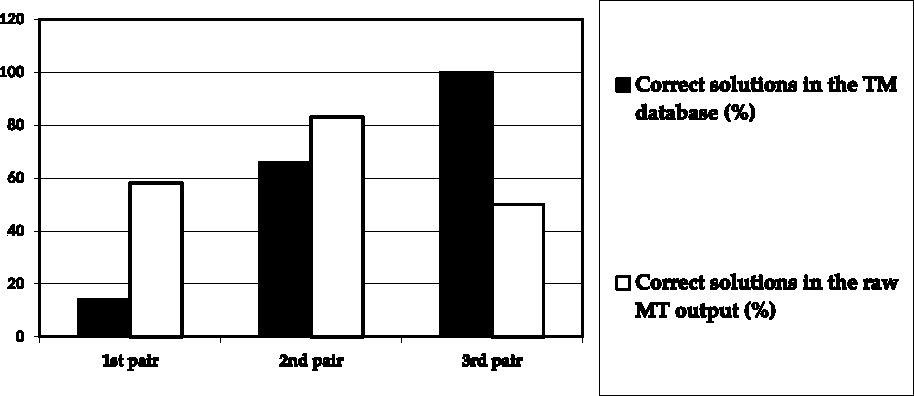
\includegraphics[width=\textwidth]{figures/rossetti-gaspari/figure1.pdf}
\caption{Percentage of correct translation solutions provided by the TM and the raw MT output}
\label{rossetti-gaspari:fig:1}
\end{figure}


Looking at these data, we can observe that, although the number of correct translation solutions provided by the TM database steadily increased as a result of the updates, in two out of three cases the percentage of correct solutions contained in the TM database was lower than the corresponding percentage contained in the raw MT output: in two out of three cases -- i.e. for the first and second pair -- post-\isi{editing} raw MT output represented the most effective option in terms of the incidence of correct translation solutions. Nonetheless, it should be noted that a larger number of correct translation solutions does not necessarily imply a lower level of perceived difficulty, nor a shorter amount of time spent on the task. Therefore, our proposed model investigates these two further aspects in \sectref{ressetti-gaspari:sec:5} and \sectref{ressetti-gaspari:sec:6}, respectively.

\section{Second set of results: Perceptions of difficulty}\label{ressetti-gaspari:sec:5}

This section deals with the level of difficulty that the participants perceived when working within the two scenarios considered; more precisely, with the perceived difficulty associated with the translation strategies -- or Internet searches -- that they had to adopt. The data on the type and frequency of translation strategies were collected by means of TAPs, while evidence on perceptions of difficulty was gathered by means of retrospective interviews.


\Citet[76]{Lorscher1991} points out that ``a translation strategy is a potentially conscious procedure for the solution of a problem which an individual is faced with when translating a text segment from one language into another''. Accordingly, in order to identify the translation strategies employed by the subjects, our analysis started from the translation problems which they verbalised and for which either the TM database or the raw MT output contained translations which needed checking by means of Internet searches. Each Internet search was assigned to a translation strategy on the basis of its purpose.

\largerpage
The classification scheme used to this end was adapted from the categorisations proposed by \citet{Krings1986Translation} and \citet{Gerloff1986}; these were partly modified on the basis of the specific phenomena which were observed during the TAP experiments conducted during this work. More precisely, the translation strategies identified were:
\begin{itemize}
 \item Equivalent retrieval -- i.e. search for a translation
 \item Equivalent monitoring -- i.e. check on a potential translation
 \item Comprehension of the source-language term
 \item Comprehension of the target-language term
 \item Contextualisation -- i.e. reproduction of stylistic features
 \item Reduction
 \item Reformulation
\end{itemize}

After performing the task assigned to him/her, each of the subjects was provided with his/her source text or raw output -- depending on the task assigned -- along with the target text he/she had delivered and a list of his/her four most frequent strategies. Next, during individual retrospective interviews, each participant was asked to rank the strategies in the order of the difficulty which he/she had perceived when adopting them, from least difficult -- ranking 1 -- to most difficult -- ranking 4; lists of the strategies most frequently adopted by the participants and their corresponding rankings can be found in Appendices C-H. The decision to focus solely on the four strategies most frequently adopted by each participant was based on the assumption that it would be easier for them to accurately retrieve this type of information, without having to remember strategies used relatively rarely during the experimental sessions.


Since difficulty is an elusive concept, the students were provided with a notion of ``difficulty'' to use as a guideline: they were asked to think about all those cases in which Internet searches having a specific purpose -- i.e. corresponding to a strategy -- had to be abandoned because they did not give the expected results. The participants were not allowed to give an equal ranking to two or more strategies. Moreover, although they were asked to rank their four most frequent strategies, the analysis took into consideration only one strategy, namely the one which each subject had adopted most often and that, as a result, corresponded to the relative majority of his/her Internet searches. It was assumed that, by focusing on the strategy which each subject had employed most often in the experimental sessions, it would be possible to gather data on the difficulty perceived during most phases of the translation with TM software or the PE processes. Subsequently, by adopting the model proposed in this pilot study, we could check the extent to which the number of correct solutions impacted on the \isi{perception} of difficulty.


As far as the TM working scenario is concerned, \tabref{rossetti-gaspari:tab:3} shows the data referring to the percentage of correct solutions provided by the TM database in relation to the translation problems verbalised in each of the three sessions, the strategy most frequently adopted by each subject and the corresponding ranking assigned to this strategy on the basis of the level of difficulty perceived when employing it.

\begin{table}[t]
\caption{Percentage of correct solutions provided by the TM database, most frequent strategies and their rankings in terms of perceived difficulty}
\label{rossetti-gaspari:tab:3}
\begin{tabularx}{\textwidth}{lrQr}
\lsptoprule
 \parbox{1.5cm}{Sessions using TM} &
 \parbox{5cm}{\raggedright Percentage of correct translation solutions -- out of the overall translation problems identified} &
 \parbox{2cm}{\raggedright Most frequently adopted strategy} &
 \parbox{2.2cm}{\raggedright Ranking --out\newline of 4-- of perceived difficulty}\\
 \midrule
  1\textsuperscript{st} session &  14\% & Equivalent retrieval
  \newline -- used 22
  out of 49 times &  4\\
  
  \tablevspace
  2\textsuperscript{nd} session &  66\% & Equivalent monitoring
 \newline -- used 4 out of 8 times &  3\\
  
  \tablevspace
  3\textsuperscript{rd} session &  100\% & Equivalent monitoring
  \newline-- used 7
  out of 10 times &  3\\
\lspbottomrule
\end{tabularx}
\end{table}

The data show that:
\begin{itemize}
 \item as the sessions took place, there was a change in the type of strategy most frequently adopted by the subjects;
 \item the ranking of perceived difficulty assigned to the strategy of \isi{equivalent retrieval} was higher than the ranking assigned to the strategy of \isi{equivalent monitoring}.
\end{itemize}

\clearpage
The shift from the strategy of \isi{equivalent retrieval} -- the most used during the first session -- to that of \isi{equivalent monitoring} -- the most employed during the second and third sessions -- can be assumed to be a result of the steady updating of the TM database: the participants were provided with an ever-increasing number of solutions previously inserted by their colleagues working on similar texts. As a result, even when they were not sure about the correctness of a translation solution, they were led to employ it as a starting point for their searches, instead of looking for equivalents from scratch. This shift led to a decrease in the level of difficulty perceived during the majority of the Internet searches performed, thus reducing the overall difficulty associated with the \isi{translation process} when using TM software.


With regard to the PE scenario, \tabref{rossetti-gaspari:tab:4} shows data regarding the percentage of correct translation solutions provided by the MT output in relation to the translation problems verbalised within each session, the strategy most frequently adopted by each subject and the corresponding ranking assigned to this strategy on the basis of the level of difficulty perceived when employing it.


\begin{table}[t]
\caption{Percentage of correct solutions provided by the raw MT output, most frequent strategies and their rankings in terms of perceived difficulty}
\label{rossetti-gaspari:tab:4}
\begin{tabularx}{\textwidth}{lrQr}
\lsptoprule
  \parbox{1.5cm}{\raggedright Sessions with full MT PE} &
  \parbox{4cm}{\raggedright Percentage of correct translation solutions -- out of the overall translation problems identified} &
 \parbox{3cm}{\raggedright Most frequently adopted strategy} &
 \parbox{2.2cm}{\raggedright Ranking --out\newline of 4-- of perceived difficulty}\\
 \midrule
  1\textsuperscript{st} session &  58\% & Contextualisation
 -- used 16
  out of 45 times &  4\\
  2\textsuperscript{nd} session &  83\% & Contextualisation
 -- used 7
  out of 15 times &  4\\
  3\textsuperscript{rd} session &  50\% & Contextualisation
 -- used 4 times
  out of 13 &  4\\
\lspbottomrule
\end{tabularx}
\end{table}

\clearpage
The data which were gathered from the three students who worked within the PE scenario show that:
\begin{itemize}
 \item there is no variation in the type of strategy which each of the participants adopted most often -- i.e. contextualisation;
 \item all three subjects gave an equal ranking to the strategy of contextualisation, which was unanimously regarded as the most difficult.
\end{itemize}

The fact that the strategy most frequently adopted by all three subjects was that of contextualisation suggests that the type of translation problem for which they were led to perform the highest number of Internet searches was the same. In those cases, they used Internet searches to look for comparable texts so as to determine whether the MT output had respected the stylistic features of the economic press release text type in the \isi{target language}. Therefore, it can be observed that, even in those cases in which the output provided solutions regarded as correct to more than half the translation problems encountered -- such as in the first and second sessions -- the solutions provided did not help the participants solve the stylistic problems identified. An in-depth knowledge of both textual and extra-textual features is necessary to reproduce the style of a specific text type -- e.g. while in English managers tend to use the pronoun ``we'' when talking about their companies, impersonal forms are more frequent in \ili{Italian}. Therefore, this may suggest that the participants were aware of the risk that the style of the MT output could be inconsistent or inadequate, for instance due to processing the text on a sentence-by-sentence basis without taking contextual knowledge or genre-specific features into account. This would explain why, unlike the participants working within the TM scenario, they did not use the stylistic features in the raw output as a starting point -- e.g. by checking whether they were correct -- but rather looked up comparable press releases written in \ili{Italian}.


To sum up, our model of data \isi{triangulation} has so far investigated whether the number of correct solutions provided by the TM and the raw MT output influenced participants' perceptions of the difficulty of the translation strategies adopted. It was observed that TM use reduced the difficulty perceived by the participants to a larger extent as far as translation strategies were concerned, because it provided the participants with an ever-increasing number of translations which could be checked instead of translated from scratch and which facilitated their Internet searches. On the contrary, with regard to the full PE setting, it was observed that the Internet searches made to enable reproduction of the stylistic features of the press release text type were experienced as the most difficult by all participants, possibly because they did not trust the raw MT output enough to use its translation solutions as starting points for their Internet search strategies. To complete our model, we also used time measurements to analyse the impact of translation solutions on the duration of the translation and the PE tasks. This part of the analysis will be addressed in the following section.


\section{Third set of results: Duration of the tasks}\label{ressetti-gaspari:sec:6}

This section compares the duration of the translation tasks using TM software and of the full PE tasks. We used the data gathered by means of TAPs and time measurements in order to check whether the number of correct translation solutions respectively provided by the TM software and the raw MT output had an impact on the time taken by the participants to complete their tasks. \tabref{rossetti-gaspari:tab:5} shows the data regarding the duration of the translation and PE processes and the percentage of correct translation solutions respectively provided by the TM database and the raw MT output to the translation problems verbalised by the participants.



\begin{table}
 \caption{Duration of the tasks and percentage of correct translation solutions}
 \label{rossetti-gaspari:tab:5}
\fittable{
  \begin{tabular}{lrrrr}
  \lsptoprule
  pair &
  \parbox{2.5cm}{\raggedright Duration of the translation process} &
  \parbox{2.7cm}{\raggedright Percentage of correct solutions in the TM\vphantom{j}} & 
  \parbox{2cm}{\raggedright Duration of the PE process} & 
  \parbox{3.2cm}{\raggedright Percentage of correct solutions in the raw MT output}\\
  \midrule
    1\textsuperscript{st}  & 52 min &  14\% &  50 min &  58\%\\
    2\textsuperscript{nd}  & 22 min & 66\% &  24 min &  83\%\\
    3\textsuperscript{rd} & 17 min & 100\% &  27 min &  50\%\\
  \lspbottomrule
  \end{tabular}
}
\end{table}

As can be observed in \tabref{rossetti-gaspari:tab:5}, in two out of three cases -- i.e. for the second and third pair of participants -- using a TM was the most effective option timewise. In addition, these data show that translating using a TM database providing an ever-increasing number of correct translation solutions resulted in a steady reduction in the time employed by the participants. In contrast, a higher number of correct translation solutions did not necessarily imply a shorter duration for the PE task. As a matter of fact, the length of the task did not seem to be affected by the number of correct translation solutions contained in the raw MT output. To give just one example, the participant in the first pair needed more time to post-edit the text than the participant in the third pair, even though the former identified a higher percentage of correct translation solutions than the latter. This may be due to the fact that, regardless of the number of translation solutions deemed to be correct, for those cases in which the participants had to resort to Internet searches, the searches performed turned out to be time-consuming. Another reason may be the fact that the participants were wary of the solutions in the raw output. 

\section{Discussion of the findings}\label{ressetti-gaspari:sec:7}

\largerpage
As we stated in \sectref{ressetti-gaspari:sec:1}, this work was conducted on a small scale, therefore our results are preliminary in nature. When looking solely at the number of correct translation solutions, it emerged that the TM provided more correct solutions than the raw MT output only after its second update, namely to the participant of the third pair. Nonetheless, within the TM scenario, the steady increase in the number of correct solutions had an impact on the duration of the task, on the translation strategy adopted with the highest frequency and on the level of difficulty associated with it, thus leading the participants to save an increasing amount of time and to perceive a progressively lower level of difficulty. On the contrary, within the PE setting, the variations in the number of correct translation solutions contained in the raw MT output had no impact on the time employed by the participants, on the translation strategy adopted most often and on the level of difficulty assigned to it.


These preliminary findings indicate that, in addition to the number of correct translation solutions, further factors should be taken into account to model the differences in terms of perceived difficulty and time required between the translation assisted by TM software and the PE scenarios. In particular, the subjects' opinions on the translation technology being used may have influenced the dependent variables under investigation. More precisely, the participants post-\isi{editing} seemed to show a lower sense of trust in the translations contained in the raw MT output: either they did not regard this translation technology as being able to solve specific types of problems -- e.g. stylistic ones -- and therefore translated from scratch or, even when they just wanted to check whether the solution in the raw output was correct, the searches which they performed were more time-consuming. These preliminary results corroborate the notion that the relation between translators and translation technologies -- and, in particular, MT -- is very complex, as translators need to feel that they can fully trust the tool that they are using before accepting its solutions. The idea of employing translation solutions which are the result of a machine rather than a colleague's work -- who would have used his/her expertise and common sense -- may, therefore, involve too much risk for many.


 
This finding in itself points to the didactic implications of this pilot study. All the trainee translators involved in this experiment had been exposed to hands-on training in both TM software and MT post-\isi{editing} -- with components of their courses also devoted to terminology, localisation, etc. Finally, one further aspect to consider is the fact that, for this pilot study, we asked participants to deliver a publishable, high-quality final text. This requirement is likely to have had an impact on their work. For example, we can safely assume that, if the participants post-\isi{editing} had been told to use minimal PE -- with the final target text to be used for gisting purposes -- they would have spent less time and effort on Internet searches aimed at refining the stylistic features of the final target texts. Therefore, these preliminary results should be considered as deeply influenced by the final task assigned to the participants.


\section{Conclusions and future work}\label{ressetti-gaspari:sec:8}
This paper has presented a pilot study proposing a model of data \isi{triangulation} for the analysis of the respective impact of TM use and full PE of raw MT output on trainee translators' time effectiveness and perceptions of the difficulty of the translation strategies adopted. The model is based on the combined use of TAPs, retrospective interviews and time measurement: TAPs were used to identify translation problems, the translation solutions provided by the TM and the raw MT output and regarded by the participants as correct, and the translation strategies employed; retrospective interviews were employed to gather data on the participants' perceptions of the difficulty of the translation strategies adopted, while time measurement allowed us to objectively compare the duration of the translation and PE tasks.


A number of limitations can be identified in this pilot study. First of all, the sample of participants was very small, such that individual differences may have influenced the preliminary findings presented here. Secondly, the passages used belonged to only one text type and were very short; therefore, they presented a limited number of linguistic features and potential translation problems. Accordingly, this does not allow us to generalise our findings to other text types or genres. In addition, this pilot study concentrated solely on the language combination English—\ili{Italian}, and the participants translated and post-edited from English into their native \ili{Italian}. A further limitation arises from the fact that the TM database was steadily updated as the sessions progressed; therefore, three participants worked within an ever-changing scenario. Nonetheless, translating with the help of a TM database without taking advantage of this distinctive feature would have created an artificial working scenario. In addition, these preliminary findings are deeply influenced by the segments with which the TM had previously been updated, as well as by the training data used for the statistical MT system employed. A further crucial limitation is connected to the lack of an objective recording tool -- such as \isi{keystroke logging} programmes or eye trackers -- which prevented us from analysing whether the subjects actually verbalised all their actions while performing the tasks. Finally, it is worth noting that, although the participants were asked to deliver publishable high-quality texts, their final \ili{Italian} translations were not evaluated, due to an exclusive focus on the processes, rather than the products, of their translations obtained with the use of TM software or PE.


These limitations reinforce the need to further test the preliminary results obtained in this pilot study and extend this line of research, applying the proposed data \isi{triangulation} model to analyse translators' activity data in other scenarios. To give just a few examples, it would be helpful to conduct similar experiments with longer texts belonging to different types and/or with a higher number of participants in order to test the wider applicability of our preliminary results. It would also be interesting to involve trainee translators studying in different institutions, in order to determine whether and how the training received in translation technologies might influence the \isi{translation process} of the participants -- indirectly testing the actual effectiveness of such training in translation technologies. Further research should also be conducted to explore the effect of switching around the translation direction, so as to observe variations in time, strategies employed and their perceived difficulty due to the effect of directionality, especially when translating into a second language, which also constitutes an interesting, and challenging, didactic activity.


Furthermore, given the importance of translators' attitudes to translation technologies which emerged from this pilot study, it would be interesting to expand the analytical model proposed here by adding focus groups or interviews to collect data specifically on the participants' opinions on translation tools. Moreover, by combining additional data gathering methodologies, it would be possible to make up for the incompleteness which often characterises the data obtained by means of TAPs and retrospective interviews; as a matter of fact, the model proposed in this initial study may easily incorporate different methodologies. Finally, it would be advisable to extend the present work also by combining the findings of this process-oriented research with an analysis of the quality of the final products. As pointed out by \citet{Guerberof2009}, the analysis of translation productivity should be done in relation to an equal level of final quality. In this study, we relied on the students to possess an a priori notion of publishable quality for their final target texts, and we assumed that they were able to achieve it equally when working with TM and when post-\isi{editing} MT output.

\section*{Acknowledgements}

This work was conducted while both authors were at the \textit{School of Foreign Languages and Literatures, Interpreting and Translation} of the \textit{University of Bologna} at Forlì (Italy). The authors would like to thank the following people: Professor Silvia Bernardini for helpful suggestions during the design stage of the study; Dr Patrick Cadwell for his help in improving the style of the manuscript; the audience at the \textit{Translation in Transition} conference (Germersheim, 29\textsuperscript{th}--30\textsuperscript{th} January 2015) at which this paper was originally presented, for their useful feedback; the anonymous students for their participation in the pilot study described and the two anonymous reviewers for their valuable comments on a previous version of this paper.

\section*{Abbreviations}

\begin{tabular}{ll}
TM  & Translation Memory \\
MT  & Machine Translation \\
PE  & Post-\isi{editing} \\
\end{tabular}
\begin{tabular}{ll}
TAPs  & Think-Aloud Protocols \\
UAD & User Activity Data\\
\\
\end{tabular}


\section*{Appendix}

\subsection*{Appendix A: Source text to be translated by the participant of the first pair}

NAME Boosts Dividend by 10 Percent \\ \\
Board Cites Earnings Outlook, Strong Cash Flow \\ \\
The NAME (NYSE: NAME) Board of Directors today increased the regular quarterly dividend by 9.6 percent to \$0.57 per share from \$0.52 on all outstanding Class A and Class B shares. The dividend is payable March 7, 2012, to shareholders of record on Feb. 21, 2012. \\ \\
``NAME turned in a great performance in 2011 despite a volatile global operating environment,'' said NAME Chairman and CEO NAME SURNAME. ``Cash flow in 2012 is expected to be strong and clearly today's decision by the Board reflects that projection.''


\subsection*{Appendix B: Raw MT output to be post-edited by the participant of the first pair}

NAME Aumenta dividendo del 10 per cento \\ \\
Consiglio Cites guadagni Outlook, Forte Cash Flow \\ \\
L'NAME (NYSE: NAME) Consiglio di Amministrazione ha aumentato oggi il dividendo trimestrale regolare del 9,6 per cento a 0,57 dollari per azione da 0,52 dollari su tutte le classi in circolazione azioni di classe A e B. Il dividendo è pagabile 7 marzo 2012, agli azionisti registrati il 21 febbraio 2012. \\ \\
``NAME ha disputato una grande prestazione nel 2011, nonostante un contesto globale volatile,'' ha dichiarato NAME Chairman e CEO NAME SURNAME. ``Il flusso di cassa nel 2012 dovrebbe essere forte e chiaramente la decisione odierna del Consiglio che riflette la proiezione.''

\subsection*{Appendix C: Rankings obtained by the participant of the first pair working within the CAT setting\footnote{In appendices C-H, strategies are put in order of ranking of perceived difficulty -- from more (4) to less difficult (1).}}

4 - Equivalent retrieval \\
3 - Contextualisation \\
2 - Equivalent monitoring \\
1 - Comprehension of the source-language term

\subsection*{Appendix D: Rankings obtained by the participant of the second pair working within the CAT setting}

4 - Equivalent retrieval \\
3 - Equivalent monitoring \\
2 - Comprehension of the target-language term \\
1 - Comprehension of the source-language term

\subsection*{Appendix E: Rankings obtained by the participant of the third pair working within the CAT setting}

4 - Comprehension of the source-language term \\
3 - Equivalent monitoring \\
2 - Contextualisation \\
1 - Equivalent retrieval

\subsection*{Appendix F: Rankings obtained by the participant of the first pair working within the PE setting}

4 - Contextualisation \\
3 - Equivalent retrieval \\
2 - Equivalent monitoring \\
1 - Comprehension of the source-language term

\subsection*{Appendix G: Rankings obtained by the participant of the second pair working within the PE setting}

4 - Contextualisation \\
3 - Equivalent retrieval \\
2 - Comprehension of the source-language term \\
1 - Comprehension of the target-language term

\subsection*{Appendix H: Rankings obtained by the participant of the third pair working within the PE setting}

4 - Contextualisation \\
3 - Equivalent retrieval \\
2 - Equivalent monitoring \\
1 - Comprehension of the source-language term

\newpage 
\sloppy
\printbibliography[heading=subbibliography,notkeyword=this]
\end{document}

% \begin{styleTCiiiTextBody}
% @incollection{Angelone2010,
% 	address = {Amsterdam},
% 	author = {Angelone, Erik},
% 	booktitle = {\textit{Translation and cognition},},
% 	editor = {Shreve, Gregory \& Angelone, Erik},
% 	pages = {17-40},
% 	publisher = {John Benjamins},
% 	title = {Uncertainty, \isi{uncertainty management} and metacognitive problem solving in the translation task},
% 	year = {2010}
% }
% \end{styleTCiiiTextBody}
% 
% \begin{stylePredefinito}
% Carl, Michael. 2012. Translog-II: A program for recording user activity data for empirical reading and writing research. In Calzolari, Nicoletta \& Choukri, Khalid \& Declerck, Thierry \& Uğur Doğan, Mehmet \& Maegaard, Bente \& Mariani, Joseph \& Moreno, Asunción \& Odijk, Jan \& Piperidis, Stelios (eds.), \textit{Proceedings of the 8th i}\textit{nternational c}\textit{onference on l}\textit{anguage r}\textit{esources and e}\textit{valuation (LREC 2012}), 4108-4112.
% \end{stylePredefinito}
% 
% \begin{stylePredefinito}
% @article{Carl2009,
% 	author = {Carl, Michael  and  Jakobsen, Arnt Lykke},
% 	journal = {\textit{International Journal of Speech Technology}},
% 	pages = {125-138},
% 	title = {Towards statistical modelling of translators’ activity data},
% 	volume = {12},
% 	year = {2009}
% }
% \end{stylePredefinito}
% 
% \begin{stylePredefinito}
% Carl, Michael \& García Martínez, Mercedes \& Mesa-Lao, Bartolomé \& Underwood, Nancy. 2014. CFT13: A resource for research into the post{}-\isi{editing} process. In Calzolari, Nicoletta \& Choukri, Khalid \& Declerck, Thierry \& Loftsson, Hrafn \& Maegaard, Bente \& Mariani, Joseph \& Moreno, Asunción \& Odijk, Jan \& Piperidis, Stelios (eds.), \textit{Proceedings of the 9th i}\textit{nternational c}\textit{onference on l}\textit{anguage r}\textit{esources and e}\textit{valuation (LREC 2014)}, 1757-1764.
% \end{stylePredefinito}
% 
% \textrm{Carl, Michael} \textrm{\&} \textrm{Gutermuth}, \textrm{Silke} \textrm{\&}  \textrm{Hansen-Schirra}, \textrm{Silvia}\textrm{. 2015.} \textrm{Post-editing} \textrm{m}\textrm{achine} \textrm{t}\textrm{ranslation}\textrm{:} \textrm{E}\textrm{fficiency}, \textrm{s}\textrm{trategies}\textrm{, and} \textrm{r}\textrm{evision} \textrm{p}\textrm{rocesses} \textrm{in} \textrm{p}\textrm{rofessional} \textrm{t}\textrm{ranslation} \textrm{s}\textrm{ettings}\textrm{. In}\textrm{ }\textrm{Ferreira}, \textrm{Aline} \textrm{\&}  \textrm{Schwieter}, \textrm{John} \textrm{(eds.)}, \textrm{\textit{Psycholinguistic and} }\textrm{\textit{c}}\textrm{\textit{ognitive} }\textrm{\textit{i}}\textrm{\textit{nquiries into} }\textrm{\textit{t}}\textrm{\textit{ranslation and} }\textrm{\textit{i}}\textrm{\textit{nterpreting}}, \textrm{145-174. Amsterdam: John Benjamins.}
% 
% \begin{stylePredefinito}
% @incollection{Čulo2014,
% 	address = {Newcastle upon Tyne},
% 	author = {Čulo, Oliver  and  Gutermuth, Silke  and  Hansen-Schirra, Silvia  and  Nitzke, Jean},
% 	booktitle = {\textit{Post-\isi{editing} of \isi{machine translation}: P}\textit{rocesses and applications},},
% 	editor = {O’Brien, Sharon \& Winter Balling, Laura \& Carl, Michael \& Simard, Michel \& Specia, Lucia},
% 	pages = {200-218},
% 	publisher = {Cambridge Scholars},
% 	title = {The influence of post{}-\isi{editing} on translation strategies},
% 	year = {2014}
% }
% \end{stylePredefinito}
% 
% \begin{stylePredefinito}
% @book{Ericsson1993,
% 	address = {Cambridge},
% 	author = {Ericsson, Anders K.  and  Simon, Herbert A.},
% 	publisher = {MIT Press},
% 	title = {\textit{Protocol a}\textit{nalysis:} \textit{Verbal} \textit{reports} \textit{as d}\textit{ata}. Rev. ed},
% 	year = {1993}
% }
% \end{stylePredefinito}
% 
% \begin{stylePredefinito}
% @incollection{Gerloff1986,
% 	address = {Tübingen},
% 	author = {Gerloff, Pamela},
% 	booktitle = {\textit{Interlingual and i}\textit{ntercultural c}\textit{ommunication: D}\textit{iscourse and c}\textit{ognition in t}\textit{ranslation and s}\textit{econd l}\textit{anguage a}\textit{cquisition s}\textit{tudies},},
% 	editor = {House, Juliane \& Blum-Kulka, Shoshana},
% 	pages = {243-262},
% 	publisher = {Gunter Narr},
% 	title = {Second language learners’ reports on the interpretive process: Talk-aloud protocols of translation},
% 	year = {1986}
% }
% \end{stylePredefinito}
% 
% \begin{stylePredefinito}
% @article{Guerberof2009,
% 	author = {Guerberof, Ana},
% 	journal = {\textit{Localisation Focus}},
% 	number = {1},
% 	pages = {11-21},
% 	title = {Productivity and quality in the post{}-\isi{editing} of outputs from translation memories and machine translation},
% 	volume = {7},
% 	year = {2009}
% }
% \end{stylePredefinito}
% 
% \begin{stylePredefinito}
% Hansen, Gyde. 2008. The dialogue in translation \isi{process research}. In \textit{Translation and cultural diversity}\textit{: Selected} \textit{proceedings of the XVIII FIT} \textit{world congress 2008}, 386-397. Shanghai: Foreign Language Press.
% \end{stylePredefinito}
% 
% \begin{stylePredefinito}
% @incollection{Jakobsen1999,
% 	address = {Copenhagen},
% 	author = {Jakobsen, Arnt Lykke},
% 	booktitle = {\textit{Probing the process of translation: M}\textit{ethods and results, Copenhagen Studies in Language 24},},
% 	editor = {Hansen, Gyde},
% 	pages = {9-20},
% 	publisher = {Samfundslitteratur},
% 	title = {Logging target \isi{text production} with Translog},
% 	year = {1999}
% }
% \end{stylePredefinito}
% 
% \begin{stylePredefinito}
% @incollection{Jakobsen2003,
% 	address = {Amsterdam},
% 	author = {Jakobsen, Arnt Lykke},
% 	booktitle = {\textit{Triangulating translation:} \textit{Perspectives in process oriented research},},
% 	editor = {Alves, Fabio},
% 	pages = {69-95},
% 	publisher = {John Benjamins},
% 	title = {Effects of think aloud on translation speed, \isi{revision} and segmentation},
% 	year = {2003}
% }
% \end{stylePredefinito}
% 
% \begin{stylePredefinito}
% @incollection{Jääskeläinen2000,
% 	address = {Amsterdam},
% 	author = {Jääskeläinen, Riitta},
% 	booktitle = {\textit{Tapping and m}\textit{apping the p}\textit{rocesses of t}\textit{ranslation and i}\textit{nterpreting: Outlooks on e}\textit{mpirical r}\textit{esearch},},
% 	editor = {Tirkkonen-Condit, Sonja \& Jääskeläinen, Riitta},
% 	pages = {71-82},
% 	publisher = {John Benjamins},
% 	title = {Focus on methodology in think{}-aloud studies in translating},
% 	year = {2000}
% }
% \end{stylePredefinito}
% 
% \begin{stylePredefinito}
% Koponen, Maarit \& Ramos, Luciana \& Aziz, Wilker \& Specia, Lucia. 2012. Post-\isi{editing} time as a measure of \isi{cognitive effort}. In O’Brien, Sharon \& Simard, Michel \& Specia, Lucia (eds.), \textit{Proceedings of the AMTA 2012 w}\textit{orkshop on p}\textit{ost-\isi{editing} t}\textit{echnology and p}\textit{ractice (WPTP 2012)}, 11-20.
% \end{stylePredefinito}
% 
% \begin{stylePredefinito}
% @incollection{Krings1986,
% 	address = {Tübingen},
% 	author = {Krings, Hans P},
% 	booktitle = {\textit{Interlingual and i}\textit{ntercultural c}\textit{ommunication: Discourse and c}\textit{ognition in t}\textit{ranslation and s}\textit{econd l}\textit{anguage a}\textit{cquisition s}\textit{tudies},},
% 	editor = {House, Juliane \& Blum-Kulka, Shoshana},
% 	pages = {263-276},
% 	publisher = {Gunter Narr},
% 	title = {Translation problems and translation strategies of advanced \ili{German} learners of \ili{French} (L2)},
% 	year = {1986}
% }
% \end{stylePredefinito}
% 
% \begin{stylePredefinito}
% @book{Krings2001,
% 	address = {Kent},
% 	author = {Krings, Hans P.},
% 	publisher = {Kent State University Press},
% 	title = {\textit{Repairing t}\textit{exts: Empirical} \textit{investigations} \textit{of m}\textit{achine t}\textit{ranslation p}\textit{ost{}-editing} \textit{processes}},
% 	year = {2001}
% }
% \end{stylePredefinito}
% 
% \begin{stylePredefinito}
% @article{Li2004,
% 	author = {Li, Defeng},
% 	journal = {\textit{International Journal of Applied Linguistics}},
% 	number = {3},
% 	pages = {301-313},
% 	title = {Trustworthiness of think{}-aloud protocols in the study of translation processes},
% 	volume = {14},
% 	year = {2004}
% }
% \end{stylePredefinito}
% 
% \begin{stylePredefinito}
% @book{Lörscher1991,
% 	address = {Tübingen},
% 	author = {Lörscher, Wolfgang.},
% 	publisher = {Gunter Narr},
% 	title = {\textit{Translation p}\textit{erformance,} \textit{translation} \textit{process}\textit{, and t}\textit{ranslation s}\textit{trategies: A} \textit{psycholinguistic} \textit{investigation}},
% 	year = {1991}
% }
% \end{stylePredefinito}
% 
% \begin{stylePredefinito}
% @incollection{Muñóz2010,
% 	address = {Copenhagen},
% 	author = {Muñóz Martín, Ricardo},
% 	booktitle = {\textit{Methodology, t}\textit{echnology and i}\textit{nnovation in t}\textit{ranslation p}\textit{rocess r}\textit{esearch:} \textit{A} \textit{tribute to Arnt Lykke} \textit{Jakobsen},},
% 	editor = {Mees, Inger \& Alves, Fabio \& Göpferich, Susanne},
% 	pages = {87-108},
% 	publisher = {Samfundslitteratur},
% 	title = {The way they were: Subject profiling in \isi{translation process} research},
% 	year = {2010}
% }
% \end{stylePredefinito}
% 
% \begin{stylePredefinito}
% @article{O’Brien2007,
% 	author = {O’Brien, Sharon},
% 	journal = {\textit{Perspectives: Studies in Translatology}},
% 	number = {3},
% 	pages = {185-205},
% 	title = {Eye-tracking and \isi{translation memory} matches},
% 	volume = {14},
% 	year = {2007}
% }
% \end{stylePredefinito}
% 
% \begin{stylePredefinito}
% @incollection{O’Brien2010,
% 	address = {Copenhagen},
% 	author = {O’Brien, Sharon},
% 	booktitle = {\textit{Methodology, t}\textit{echnology and i}\textit{nnovation in t}\textit{ranslation p}\textit{rocess r}\textit{esearch:} \textit{A} \textit{tribute to Arnt Lykke} \textit{Jakobsen},},
% 	editor = {Mees, Inger \& Alves, Fabio \& Göpferich, Susanne},
% 	pages = {251-266},
% 	publisher = {Samfundslitteratur},
% 	title = {Eye tracking in translation \isi{process research}: Methodological challenges and solutions},
% 	year = {2010}
% }
% \end{stylePredefinito}
% 
% \begin{stylePredefinito}
% @article{O’Brien2011,
% 	author = {O’Brien, Sharon},
% 	journal = {\textit{Machine Translation}},
% 	pages = {197-215},
% 	title = {Towards predicting post{}-\isi{editing} productivity},
% 	volume = {25},
% 	year = {2011}
% }
% \end{stylePredefinito}
% 
% \begin{stylePredefinito}
% O’Brien, Sharon \& O’Hagan, Minako \& Flanagan, Marian. 2010. Keeping an eye on the UI design of \isi{translation memory}. In Brinckman, Willem-Paul \& Neerincx, Mark (eds.), \textit{Proceedings of the 28\textsuperscript{th}} \textit{European} \textit{conference on} \textit{cognitive} \textit{ergonomics}, 187-190.
% \end{stylePredefinito}
% 
% \begin{stylePredefinito}
% O’Brien, Sharon \& Moorkens, Joss. 2014. Towards intelligent post{}-\isi{editing} interfaces. In Baur, Wolfram \& Eichner, Brigitte \& Kalina, Sylvia \& Keßler, Norma \& Mayer, Felix \& Ørsted, Jeannette (eds.), \textit{Proceedings of the XXth FIT} \textit{world} \textit{congress}, 131-137.
% \end{stylePredefinito}
% 
% \begin{stylePredefinito}
% Popović, Maja \& Lommel, Arle \& Burchardt, Aljoscha \& Avramidis, Eleftherios \& Uszkoreit, Hans. 2014. Relations between different types of post{}-\isi{editing} operations, \isi{cognitive effort} and temporal effort. In Tadić, Marko \& Koehn, Philipp \& Roturier, Johann \& Way, Andy (eds.), \textit{Proceedings of the 17th a}\textit{nnual c}\textit{onference of the European a}\textit{ssociation for m}\textit{achine t}\textit{ranslation (EAMT 14)}, 191-198.
% \end{stylePredefinito}
% 
% \begin{stylePredefinito}
% @article{Reinke2013,
% 	author = {Reinke, Uwe},
% 	journal = {Special I}\textit{ssue on} \textit{Language} \textit{Technologies} \textit{for a M}\textit{ultilingual Europe}},
% 	number = {1},
% 	pages = {27-48},
% 	title = {State of the art in \isi{translation memory} technology. \textit{Translation: Computation, C}\textit{orpora,} \textit{Cognition}\textit{},
% 	volume = {3},
% 	year = {2013}
% }
% \end{stylePredefinito}
% 
% \begin{stylePredefinito}
% @article{Seewald-Heeg2005,
% 	author = {Seewald-Heeg, Uta},
% 	journal = {\textit{MDÜ (Mitteilungen für Dolmetscher und Übersetzer)}},
% 	pages = {8-38},
% 	title = {Der Einsatz von Translation-Memory-Systemen am Übersetzerarbeitsplatz},
% 	volume = {4-5},
% 	year = {2005}
% }
% \end{stylePredefinito}
% 
% \subsection{\textmd{Specia, Lucia. 2011. Exploiting} \textmd{o}\textmd{bjective} \textmd{a}\textmd{nnotations} \textmd{for} \textmd{m}\textmd{easuring} \textmd{t}\textmd{ranslation} \textmd{p}\textmd{ost}\textmd{{}-editing} \textmd{e}\textmd{ffort}\textmd{. In Forcada}\textmd{,}\textmd{} \textmd{Mi}\textmd{kel} \textmd{\&} \textmd{Depraetere}\textmd{,}\textmd{} \textmd{Heidi} \textmd{\&} \textmd{Vandeghinste}\textmd{,}\textmd{} \textmd{Vincent}\textmd{} \textmd{(eds.)}\textmd{,} \textmd{\textit{Proceedings of the 15th} }\textmd{\textit{c}}\textmd{\textit{onference of the European} }\textmd{\textit{a}}\textmd{\textit{ssociation for} }\textmd{\textit{m}}\textmd{\textit{achine} }\textmd{\textit{t}}\textmd{\textit{ranslation (EAMT 2011)}}\textmd{,} \textmd{73-80.}}
% \begin{stylePredefinito}
% Tatsumi, Midori \& Roturier, Johann. 2010. Source text characteristics and technical and temporal post{}-\isi{editing} effort: What is their relationship?. In Zhechev, Ventsislav (ed.), \textit{Proceedings of the s}\textit{econd j}\textit{oint EM+/CNGL w}\textit{orkshop “Bringing MT to the u}\textit{ser: Research on i}\textit{ntegrating MT in the translation industry” (JEC'10)}, 43-51.
% \end{stylePredefinito}
% 
% \textrm{Tirkkonen-Condit, S}\textrm{onja}. \textrm{1989}\textrm{. Professional vs.} \textrm{non}\textrm{{}-professional} \textrm{translation}\textrm{: a} \textrm{think}\textrm{{}-aloud} \textrm{protocol study}\textrm{. In} \textrm{Séguinot}, \textrm{Candace} \textrm{(ed.)}, \textrm{\textit{The translation process}}, \textrm{73-85.} \textrm{Toront}\textrm{o: H.G. Publications.}
